\begin{figure*}[hb]
  \centering

  \begin{subfigure}[t]{0.475\tw}\centering
    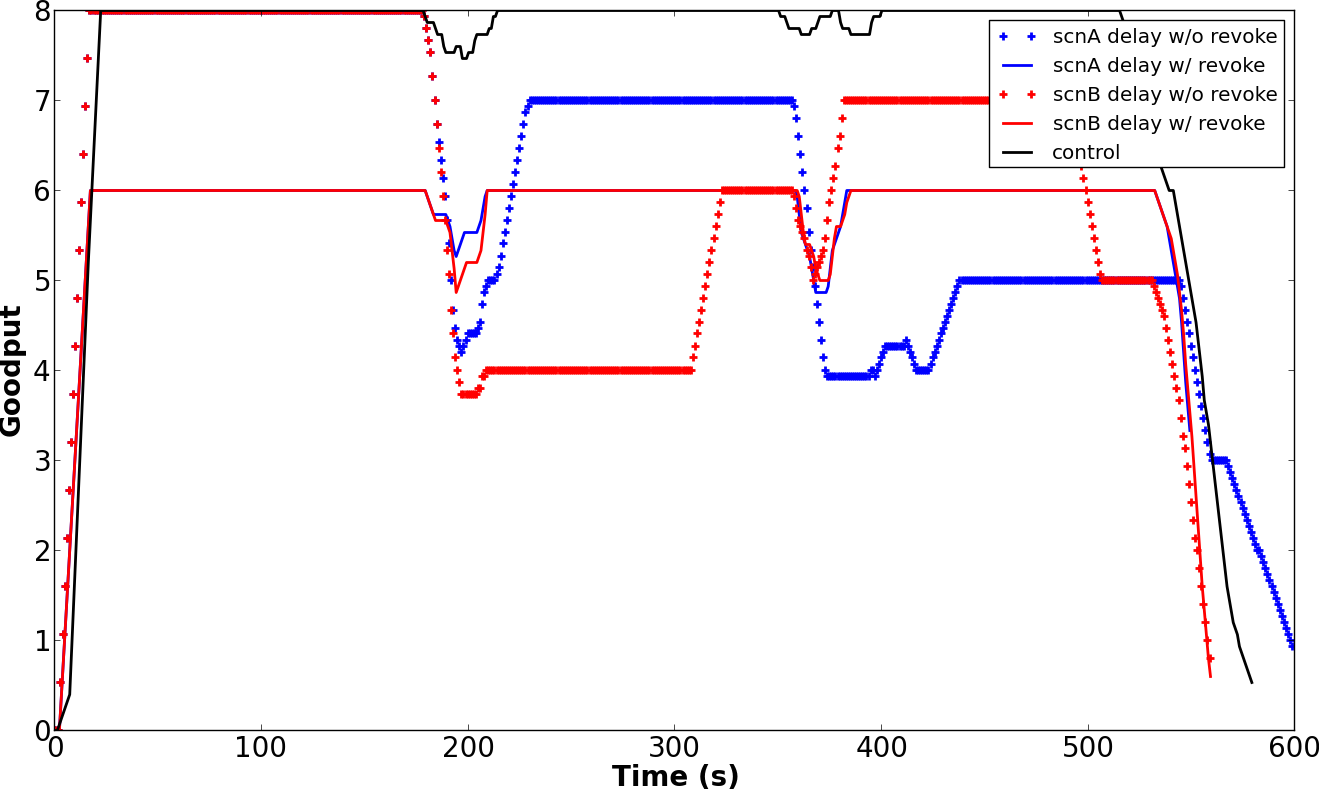
\includegraphics[width=\textwidth]{../results/control_greedy_goodput.png}
    \caption{Goodput Results for Framework 1}
    \label{fig:greedy-goodput}
  \end{subfigure}%
  \hfill
  \begin{subfigure}[t]{0.475\tw}\centering
    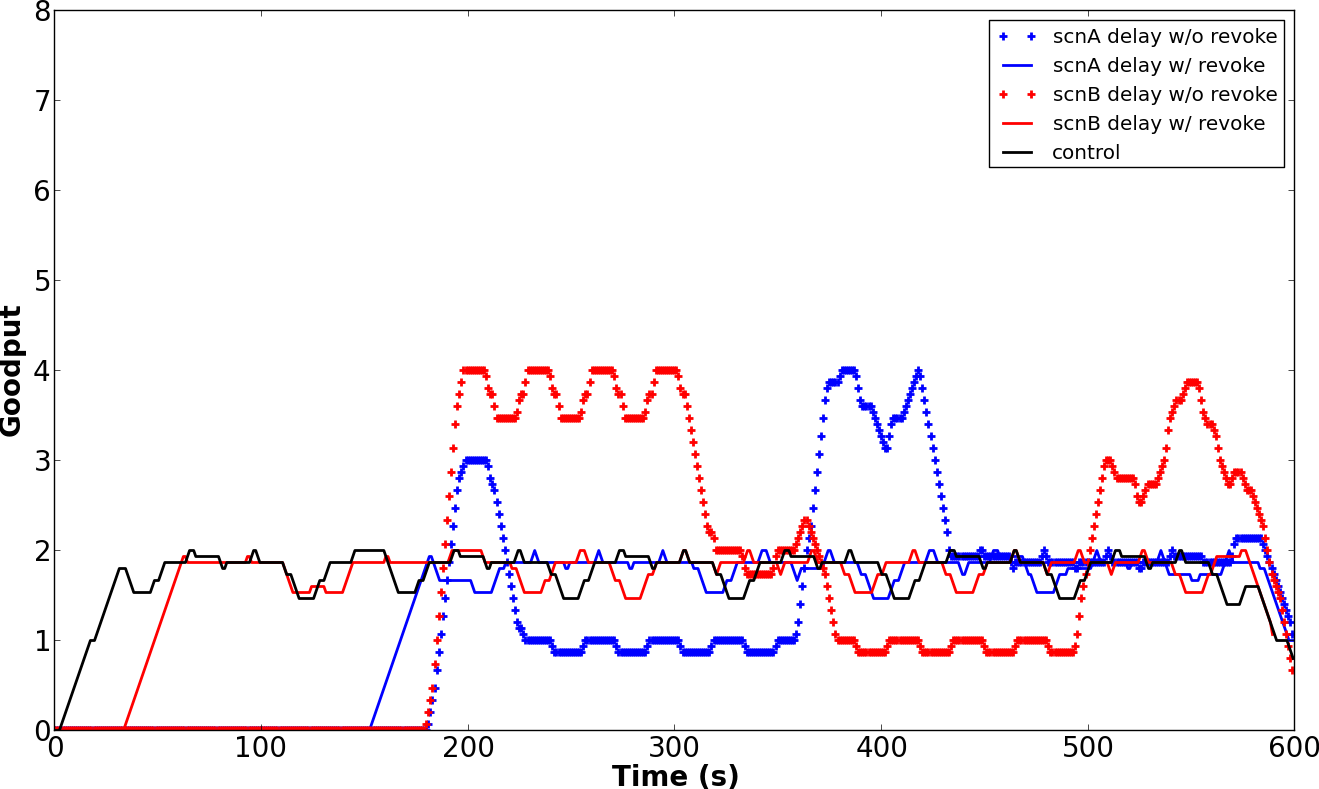
\includegraphics[width=\textwidth]{../results/control_model_goodput.png}
    \caption{Latency Results for Framework 2}
    \label{fig:model-goodput}
  \end{subfigure}%

  \caption{\textbf{Goodput Results For Frameworks A and B}
  Figure~\ref{fig:greedy-goodput} and Figure~\ref{fig:model-goodput} plots the goodput results for 
  Framework 1 and Framework 2 respectively. The black lines correspond to the case where the frameworks
  are running in isolation. The blue lines correspond to Scenario A while the red lines correspond to
  Scenario B. Solid lines correspond to the case where resource revocation is used while $+$ lines
  correspond to the case when no resource revocation is used.
  }
  \label{fig:control-goodput}
\end{figure*}
